\chapter{\texorpdfstring{Net Matrices}{Net Matrices}}
\label{ch:11}
\lecturemeta{Lezione 11 \quad\textbullet\quad 2026-07-03 \quad\textbullet\quad Roberto Bruni}{Petri nets · Esparza, \emph{Free Choice Petri Nets} (optional)}

Finora abbiamo analizzato le reti costruendone l'\textbf{occurrence graph} (\hyperref[ch:09]{09 — Occurrence Graph}, \hyperref[ch:10]{10 — Liveness}): un metodo esaustivo ma costoso, che esplode con la dimensione. Questa lezione introduce un approccio completamente diverso, \textbf{algebrico}: rappresentiamo la rete come una \textbf{matrice} e le sue computazioni come \textbf{operazioni tra vettori}. Il vantaggio è enorme — potremo dimostrare proprietà (boundedness, ripetibilità) con semplici calcoli di algebra lineare, senza costruire lo spazio degli stati.

Ripasso minimo di algebra lineare che useremo: un \textbf{vettore} su un insieme finito $E = \{e_1, \dots, e_n\}$ è una mappa $v : E \to \mathbb{Q}$ (o $\mathbb{N}, \mathbb{Z}$), scritta

\[
v = [v(e_1), \dots, v(e_n)]
\]

useremo la stessa notazione per vettori riga e colonna. Il \textbf{prodotto scalare} di due vettori è

\[
x \cdot y = \sum_i x_i y_i
\]

Confronti tra vettori:

\[
\begin{aligned}
v \le w &\quad \text{se } v(e) \le w(e) \text{ per ogni } e \\
v < w &\quad \text{se } v \le w \text{ ma diversi} \\
v \prec w &\quad \text{se } v(e) < w(e) \text{ per \textit{ogni} } e
\end{aligned}
\]

\section{\texorpdfstring{L'idea: la marcatura come vettore, il firing come somma}{L'idea: la marcatura come vettore, il firing come somma}}

Il primo passo è ovvio: una marcatura $M : P \to \mathbb{N}$ è già un vettore, di lunghezza $n = |P|$. Per esempio

\[
M_0 = [4, 0, 1, 0, 0]
\]

dice "4 token in $p_1$, uno in $p_3$".

Il passo decisivo è un'osservazione sul firing:

\begin{boxtip}{L'osservazione chiave}
La \textbf{variazione} del numero di token in un place $p$ causata dallo scatto di una transizione $t$ \textbf{non dipende dalla marcatura corrente}. È determinata \textbf{interamente dalla rete} (dalla flow relation). Quindi possiamo pre-calcolare, una volta per tutte, l'effetto di ogni transizione su ogni place — ed è proprio quello che farà la matrice.
\end{boxtip}

Per capire \emph{quale} variazione, guardiamo i \textbf{quattro modi} in cui un place $p$ e una transizione $t$ possono essere collegati:

\begingroup\small
\begin{tabularx}{\linewidth}{>{\raggedright\arraybackslash}X>{\raggedright\arraybackslash}X>{\raggedright\arraybackslash}X}
\toprule
\textbf{Connessione} & \textbf{Significato} & \textbf{Effetto su $p$} \\
\midrule
$(p,t) \notin F$ e $(t,p) \notin F$ & del tutto scollegati & \textbf{0} \\
$(p,t) \in F$ e $(t,p) \notin F$ & $p$ è solo input di $t$: serve un token, consumato & \textbf{−1} \\
$(p,t) \notin F$ e $(t,p) \in F$ & $p$ è solo output di $t$: viene prodotto un token & \textbf{+1} \\
$(p,t) \in F$ e $(t,p) \in F$ & $p$ è input \emph{e} output (self-loop): serve un token ma non cambia il totale & \textbf{0} \\
\bottomrule
\end{tabularx}
\endgroup

Questi valori $\{-1, 0, +1\}$ sono esattamente le entrate della matrice di incidenza.

\begin{boxdefinition}{Incidence matrix}
Data una rete $N = (P, T, F)$, la sua \textbf{matrice di incidenza} $\mathbf{N} : (P \times T) \to \{-1, 0, +1\}$ è definita da: \(\mathbf{N}(p, t) = \begin{cases} -1 & \text{se } (p,t) \in F \wedge (t,p) \notin F \\ +1 & \text{se } (p,t) \notin F \wedge (t,p) \in F \\ 0 & \text{altrimenti (scollegati oppure self-loop)} \end{cases}\) È una matrice con $n$ \textbf{righe} (una per place) e $m$ \textbf{colonne} (una per transizione).
\end{boxdefinition}

\begin{boxwarning}{La matrice perde i self-loop}
Attenzione al caso $0$ per il \textbf{self-loop} ($p$ sia input sia output di $t$): la matrice registra solo la \emph{variazione netta}, che è zero, quindi \textbf{non distingue} un self-loop da "nessun collegamento". Questa perdita d'informazione è la ragione per cui l'approccio algebrico, pur potente, non cattura \emph{tutto} il comportamento della rete.
\end{boxwarning}

Ogni \textbf{colonna} della matrice è il vettore $\vec{t_j}$ (l'effetto della transizione $t_j$ su tutti i place); ogni \textbf{riga} è il vettore $p_i$ (l'effetto di tutte le transizioni sul place $p_i$).

\subsection{\texorpdfstring{Esempio: distributore automatico}{Esempio: distributore automatico}}

\begin{figure}[!htb]
\centering
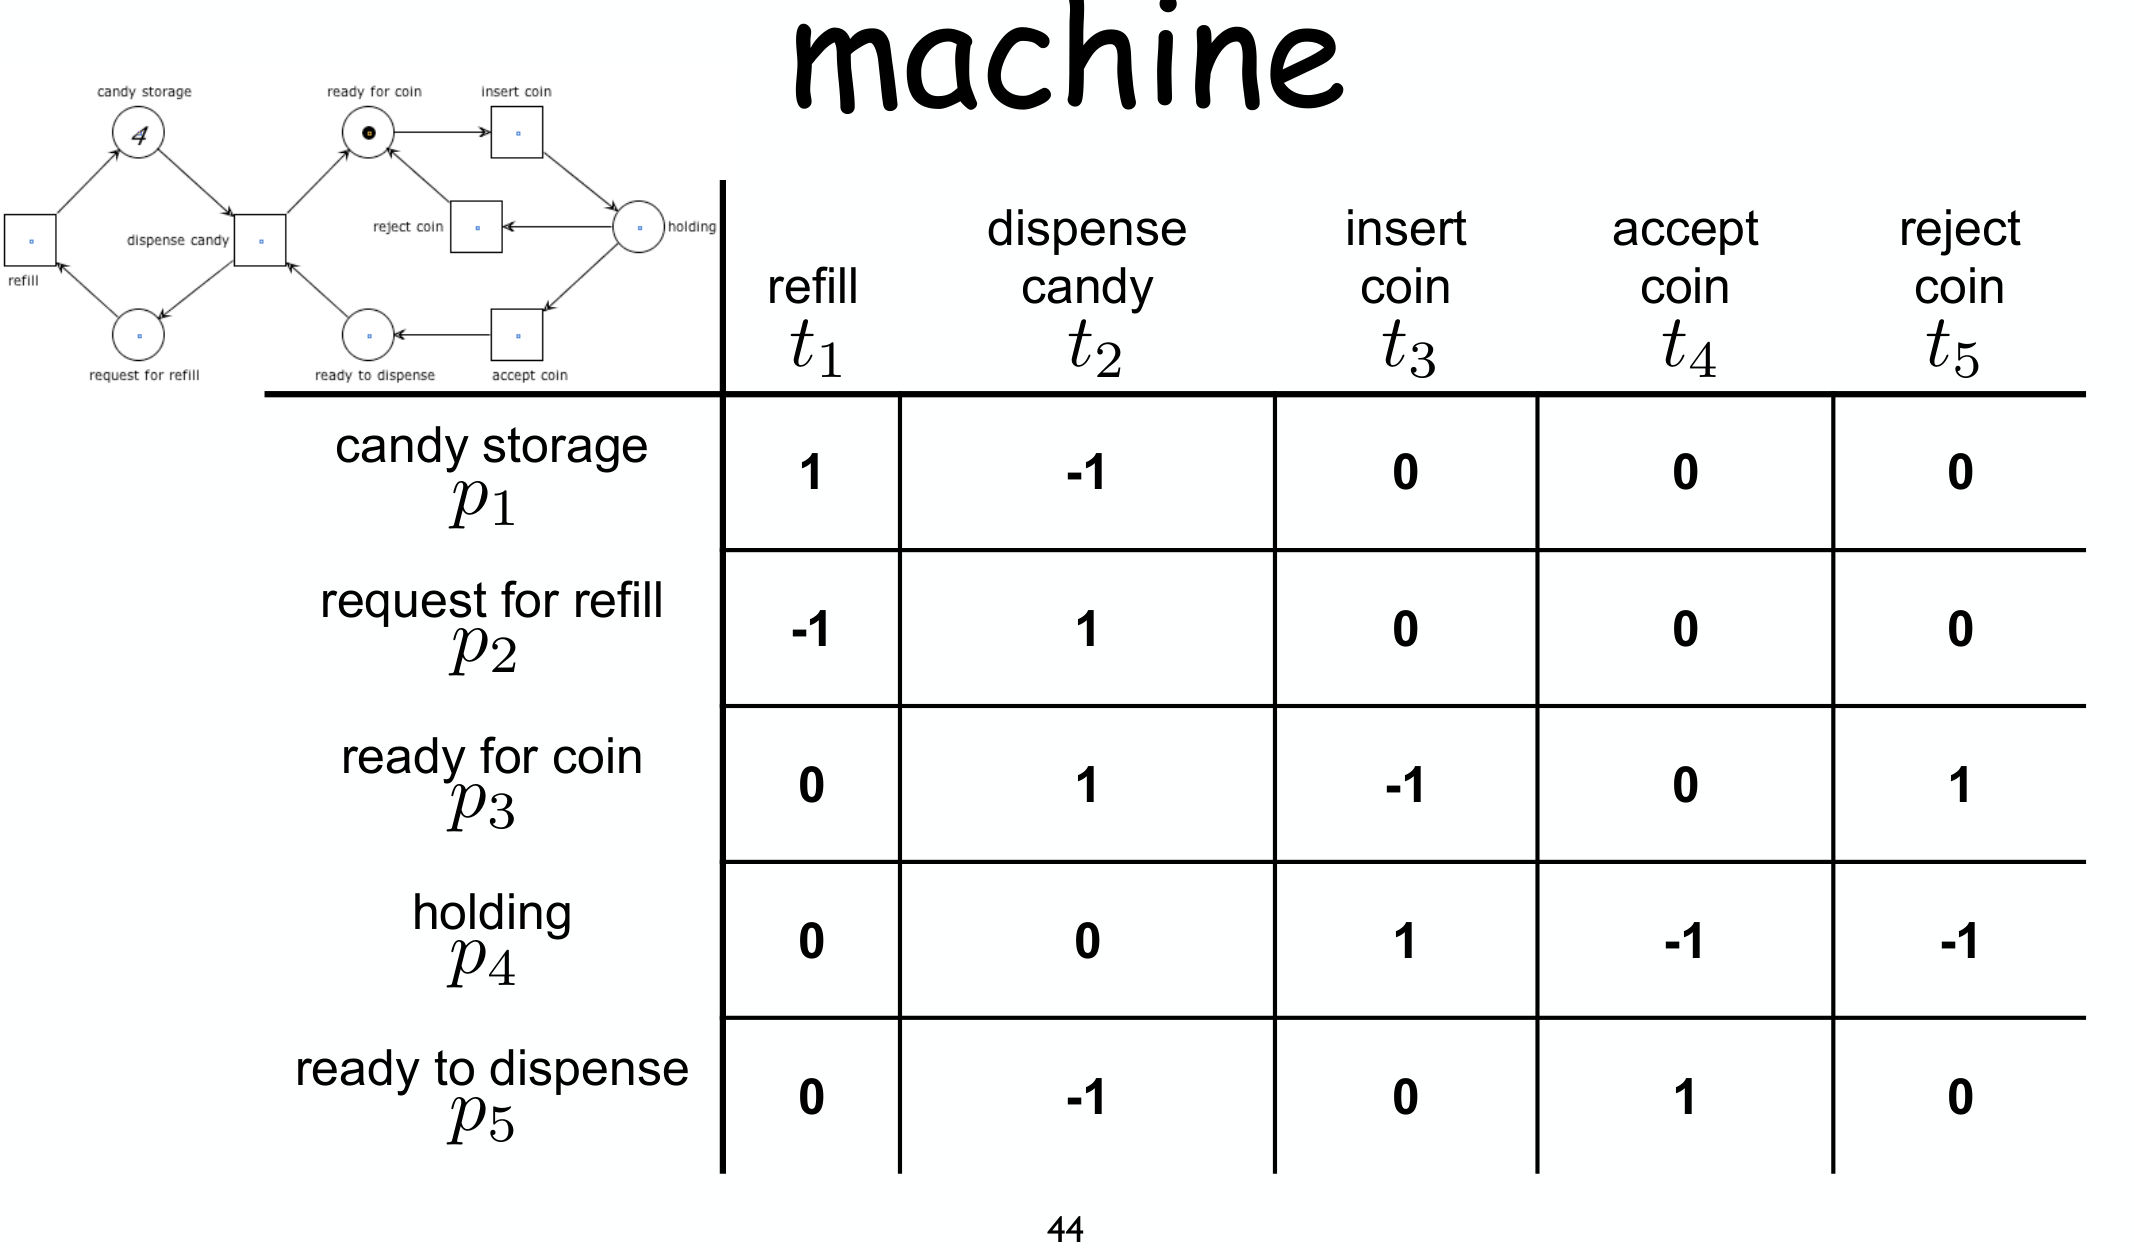
\includegraphics[width=0.74\linewidth,height=0.34\textheight,keepaspectratio]{images/11-net-matrices_p42_vending-incidence.png}
\caption{Vending machine e la sua matrice di incidenza. Ogni cella $\mathbf{N}(p_i, t_j)$ dice come lo scatto di $t_j$ modifica il numero di token in $p_i$: per esempio la colonna di \texttt{refill} ($t_1$) è $[+1, -1, 0, 0, 0]$ (produce candy storage, consuma request for refill).}
\end{figure}

\section{\texorpdfstring{Il firing come operazione vettoriale}{Il firing come operazione vettoriale}}

Con la matrice, lo scatto di una singola transizione diventa una \textbf{somma di vettori}. Se $M \xrightarrow{t} M'$, allora

\[
M' = M + \vec{t}
\]

dove $\vec{t}$ è la colonna di $t$ nella matrice di incidenza. Per esempio, dalla marcatura $M_0 = [4,0,1,0,0]$ lo scatto di $t_3$ (colonna $[0,0,-1,1,0]$) porta a

\[
M_1 = [4,0,0,1,0]
\]

Per gestire \emph{sequenze} di scatti serve un modo di sommare tutti gli effetti in un colpo solo. La chiave è contare quante volte scatta ciascuna transizione, ignorando l'ordine.

\begin{boxdefinition}{Parikh vector}
Data una sequenza $\sigma \in T^\star$, il suo \textbf{Parikh vector} $\vec{\sigma} : T \to \mathbb{N}$ associa a ogni transizione $t$ il \textbf{numero di sue occorrenze} in $\sigma$. Per una singola transizione, $\vec{t}$ è il vettore con un $1$ nella posizione di $t$ e $0$ altrove. Definizione ricorsiva: \(\vec{\epsilon} = \mathbf{0} \qquad \overrightarrow{\sigma t} = \vec{\sigma} + \vec{t}\)
\end{boxdefinition}

Per esempio, se $\sigma = t_3 t_5 t_3 t_4 t_2$, il Parikh vector è

\[
\vec{\sigma} = [0, 1, 2, 1, 1]
\]

(zero $t_1$, un $t_2$, due $t_3$, un $t_4$, un $t_5$). \textbf{Il Parikh vector dimentica l'ordine} — ed è esattamente ciò che ci serve.

Combinando matrice e Parikh vector otteniamo il risultato centrale della lezione. Il legame parte da un fatto di algebra lineare: \textbf{moltiplicare la matrice $\mathbf{N}$ per il Parikh vector di una singola transizione seleziona la colonna di quella transizione}. Infatti $\vec{t}$ ha un solo $1$ (nella posizione di $t$) e zeri altrove, quindi

\[
\mathbf{N} \cdot \vec{t}
\]

estrae esattamente la colonna $\vec{t}$ della matrice — cioè l'effetto di $t$. Ma allora il singolo scatto $M \xrightarrow{t} M' = M + \vec{t}$ si riscrive come

\[
M' = M + \mathbf{N} \cdot \vec{t}
\]

è già la marking equation per una sequenza lunga uno. Per induzione la si estende a sequenze qualsiasi.

\begin{boxtheorem}{Marking equation lemma}
Se $M \xrightarrow{\sigma} M'$, allora \(M' = M + \mathbf{N} \cdot \vec{\sigma}\) \emph{Dimostrazione (induzione sulla lunghezza di $\sigma$).}

\textbf{Base} ($\sigma = \epsilon$): \(\vec{\sigma} = \mathbf{0} \implies M' = M\) banalmente vero.

\textbf{Passo} ($\sigma = \sigma' t$): sia $M \xrightarrow{\sigma'} M'' \xrightarrow{t} M'$. Allora \( \begin{aligned} M' &= M'' + \mathbf{N}\cdot\vec{t} \\ &= (M + \mathbf{N}\cdot\vec{\sigma'}) + \mathbf{N}\cdot\vec{t} \\ &= M + \mathbf{N}\cdot(\vec{\sigma'} + \vec{t}) \\ &= M + \mathbf{N}\cdot\vec{\sigma} \end{aligned} \) $\blacksquare$
\end{boxtheorem}

\begin{figure}[!htb]
\centering
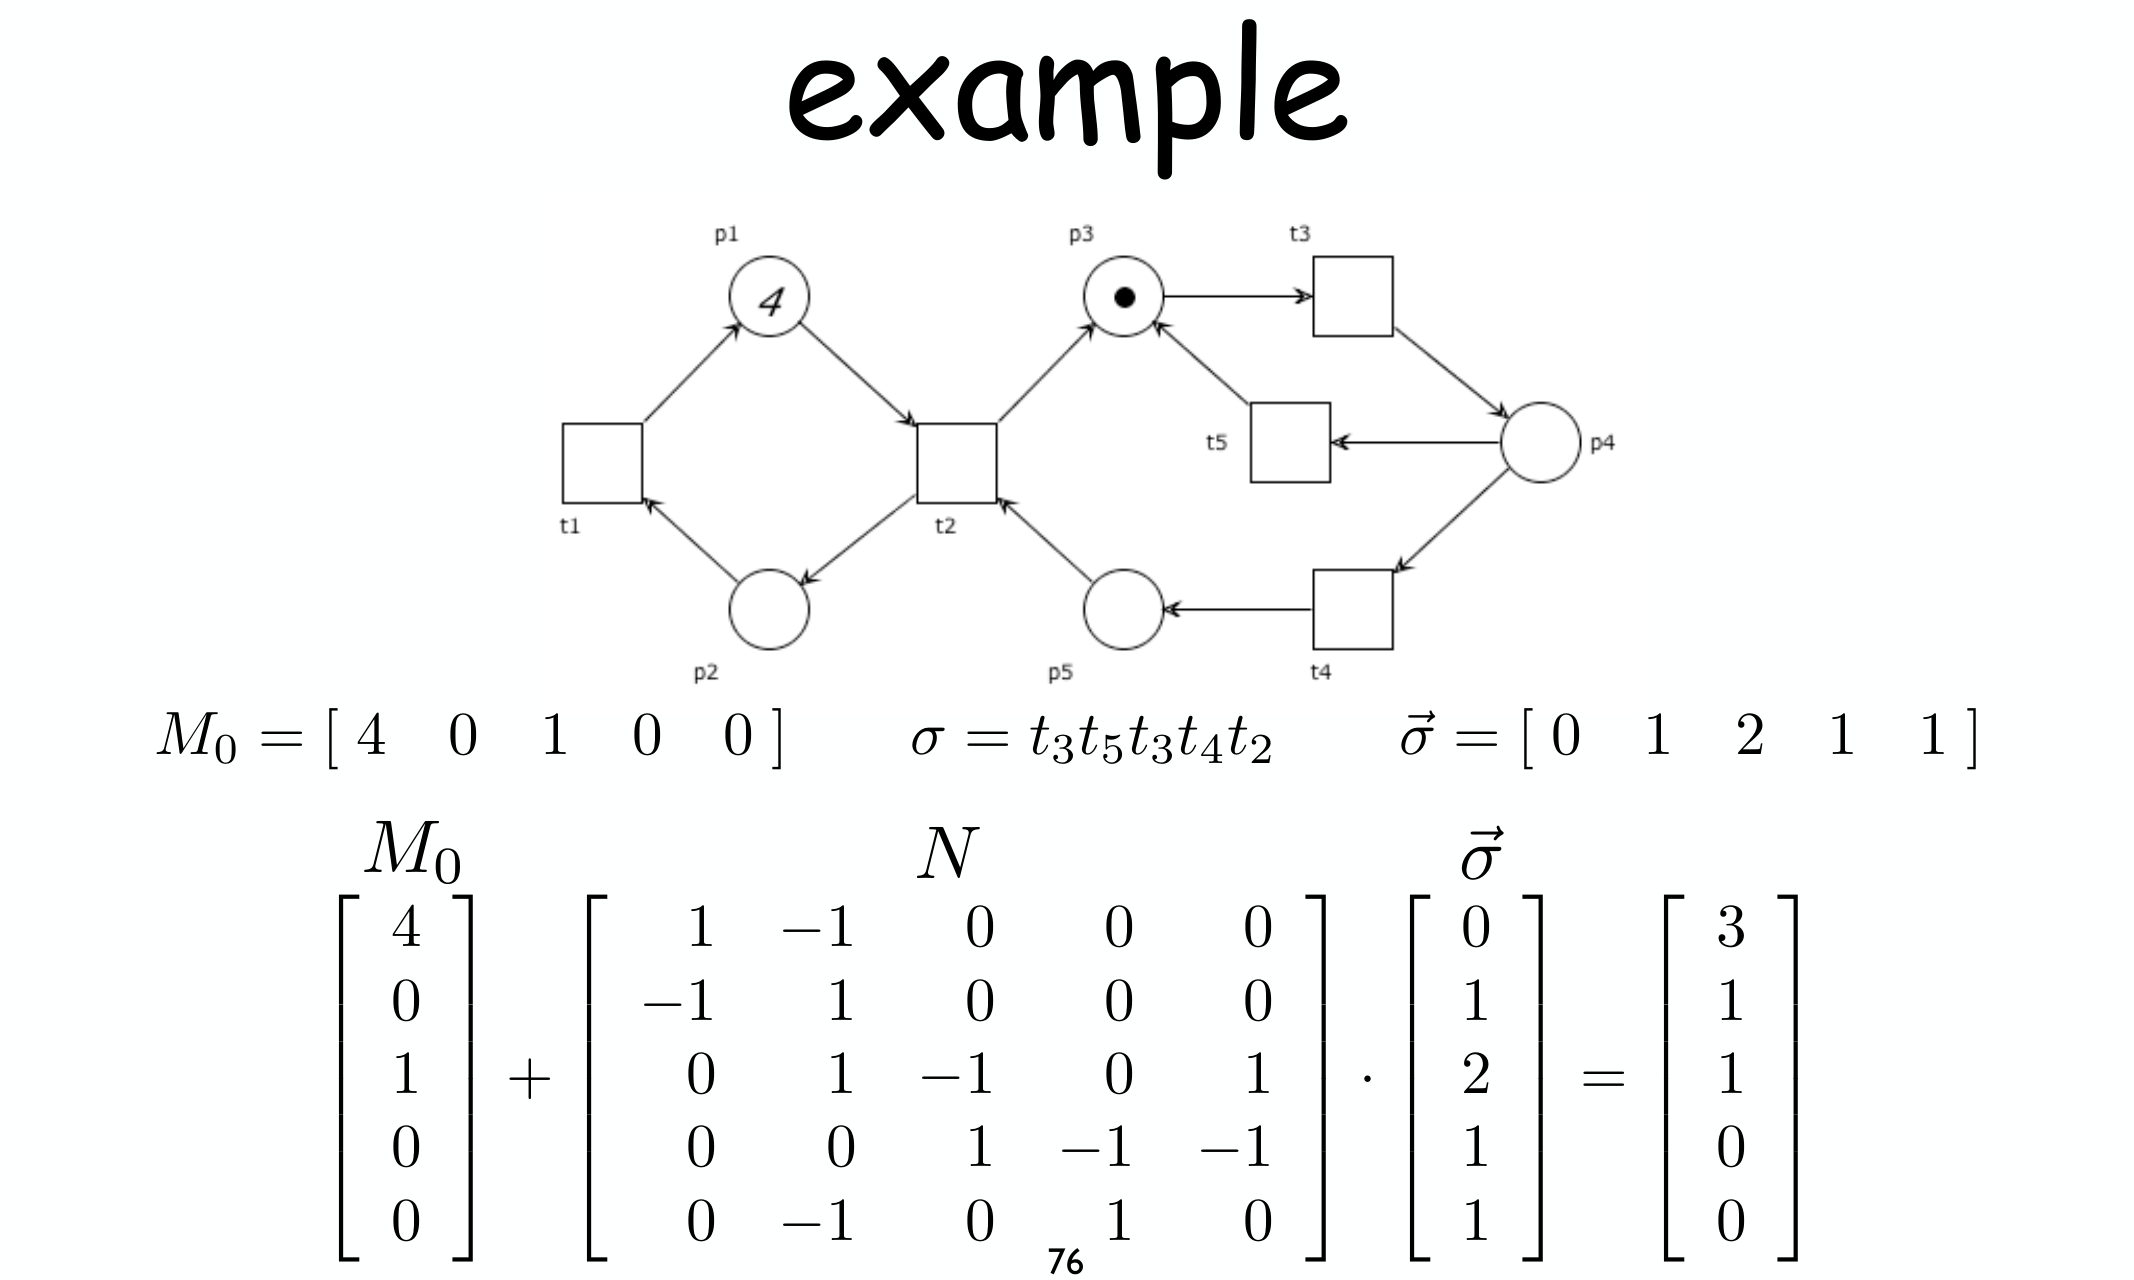
\includegraphics[width=0.74\linewidth,height=0.34\textheight,keepaspectratio]{images/11-net-matrices_p74_marking-equation.png}
\caption{Marking equation in azione. La marcatura finale $[3,1,1,0,0]$ si ottiene con \textbf{una moltiplicazione matrice-vettore} $\mathbf{N} \cdot \vec{\sigma}$ sommata a $M_0$, senza simulare i cinque scatti uno per uno.}
\end{figure}

\begin{boxnote}{La conseguenza sorprendente}
La marcatura raggiunta da una sequenza dipende \textbf{solo dal numero di occorrenze} di ciascuna transizione, \textbf{non dall'ordine} in cui scattano. Quindi \textbf{ogni permutazione eseguibile} delle stesse transizioni porta alla \textbf{stessa} marcatura. (L'ordine conta per stabilire se la sequenza è \emph{eseguibile}, ma non per il risultato finale.)
\end{boxnote}

\begin{boxwarning}{Il lemma è una condizione necessaria, non sufficiente}
Il marking equation lemma vale \emph{se} $M \xrightarrow{\sigma} M'$. Il calcolo \(M + \mathbf{N}\cdot\vec{\sigma}\) si può però fare per qualsiasi $\vec{\sigma}$: se il risultato ha una componente \textbf{negativa}, la sequenza \textbf{non è eseguibile} (non si può avere un numero negativo di token). Questo è un test veloce di \emph{non-eseguibilità}: un valore $\ge 0$ ovunque \emph{non} garantisce l'eseguibilità (l'ordine potrebbe non funzionare), ma un valore negativo la esclude di sicuro.
\end{boxwarning}

\section{\texorpdfstring{La monotonicità e i suoi corollari}{La monotonicità e i suoi corollari}}

Dalla marking equation discende una proprietà fondamentale: aggiungere token "in più" non toglie possibilità.

\begin{boxtheorem}{Monotonicity lemma}
Se $M \xrightarrow{\sigma} M'$, allora \(M + L \xrightarrow{\sigma} M' + L\) per \textbf{qualsiasi} vettore $L$. (Vale anche per sequenze infinite.)

\emph{Idea:} per induzione, usando la marking equation a ogni passo: se $M''$ abilita $t$, allora $M'' + L$ abilita $t$ (ha \emph{almeno} gli stessi token), e lo scatto produce \(M'' + L + \mathbf{N}\cdot\vec{t} = M' + L\)
\end{boxtheorem}

\begin{boxtip}{Cosa dice, intuitivamente}
\begin{itemize}
\item Se certe attività si possono fare con \textbf{meno} risorse, allora si possono fare anche con \textbf{più} risorse.
\item Se le eseguiamo con \textbf{risorse in più} del necessario, quelle risorse extra vengono \textbf{conservate} (restano lì alla fine, come il $+L$).
\end{itemize}
\end{boxtip}

Da qui seguono tre lemmi che collegano l'algebra alle proprietà comportamentali.

\begin{boxtheorem}{Corollario: ripetibilità}
Se $M \xrightarrow{\sigma} M'$ con $M \subseteq M'$, allora \(M \xrightarrow{\sigma\sigma\sigma\cdots}\) (la sequenza si può ripetere all'infinito).

Il "surplus" \(L = M' - M \ge 0\) prodotto dal primo giro, per monotonicità, basta e avanza per far ripartire $\sigma$ da capo, all'infinito.
\end{boxtheorem}

\begin{boxtheorem}{Boundedness lemma}
Se un sistema è \textbf{bounded} e $M \in [M_0\rangle$ con $M \supseteq M_0$, allora \(M = M_0\)

\emph{Idea:} se fosse $M = M_0 + L$ con $L \ne \mathbf{0}$, per monotonicità potremmo raggiungere \(M_0 + kL \quad \text{per ogni } k\) accumulando token senza limite — contraddicendo la boundedness.

\textbf{Conseguenza operativa:} se troviamo una marcatura raggiungibile $M \supset M_0$ (strettamente maggiore dell'iniziale), il sistema è \textbf{unbounded}. È il criterio algebrico dietro il coverability graph di \hyperref[ch:09]{09 — Occurrence Graph}.
\end{boxtheorem}

\begin{boxtheorem}{Repetition lemma}
Se $M \xrightarrow{\sigma} M'$ e $M \xrightarrow{\sigma\sigma\cdots}$ (ripetibile all'infinito), allora \(M \subseteq M'\)

\textbf{Conseguenza:} se una sequenza $\sigma$ si può eseguire un numero arbitrario di volte, allora $\sigma$ \textbf{produce almeno tante risorse quante ne consuma} (altrimenti, ripetendola, prima o poi un place andrebbe sotto zero). Combinato col corollario precedente, si ha: \(\sigma \text{ ripetibile all'infinito} \iff M \subseteq M'\)
\end{boxtheorem}

Con l'algebra delle matrici abbiamo strumenti per ragionare sulle reti \textbf{senza} costruire l'occurrence graph: la marking equation calcola dove si arriva, la monotonicità e i suoi lemmi caratterizzano ripetibilità e boundedness. Nelle prossime lezioni useremo questi risultati per la nozione di \textbf{soundness} dei workflow net. $\rightarrow$ \hyperref[ch:12]{12 — Soundness}